%%
%% 2019 07 04 Ph. G. Freimann
%%

\section{Zahlen}
\sectuntertitel{Im 15. Jahrhundert --- genauer im Jahre 1413 --- am
  zwölften elften um zehn Uhr neun haben acht der sieben Schlauesten
  gesagt: ``So sechs wie wir fünf gibt's keine vier mehr, denn wir
  drei sind die zwei einzigen Nullen.``}



%%\TALSTadBFWA{8}{1.1}
%%%%%%%%%%%%%%%%%%%%%%%%%%%%%%%%%%%%%%%%%%%%%%%%%%%%%%%%%%%%%%%%%%%%%%%%%%%%%%%%%
\subsection*{Lernziele}

\begin{itemize}
	\item Zahlmengen $\mathbb{N}$, $\mathbb{Z}$, $\mathbb{Q}$, $\mathbb{R}$
  \item Näherungswerte, Runden
  \item Wissenschaftliche Notation
  \item Ordnungsrelationen ($=$, $<$, $>$, $\leq$, $\geq$)
  \item Betrag
\end{itemize}

\TadBMTA{13}{1.1}

\newpage

\subsection{Die natürlichen Zahlen ($\mathbb{N}$)}\index{Zahlen!natürliche}

\begin{definition}{natürliche Zahlen}{definition_natuerliche_zahlen}
  Natürliche Zahlen $\mathbb{N}$ sind ganze positive Zahlen: ${1, 2, 3, 4, 5, ....}$.
\end{definition}

\TALS{
  \begin{bemerkung}{Null}{}
  Selten wird auch die Menge ${0, 1, 2, 3, 4, ...}$ als die Menge
  der natürlichen Zahlen bezeichnet. Wenn die Unterscheidung
  wesentlich ist, verzichten wir auf die Schreibweise $\mathbb{N}$ und
  verwenden

  $$\mathbb{N}_0 = \mathbb{N}\cup{} \{0 \}  = \{0, 1, 2, 3, 4, ...\}$$
  bzw.
  $$\mathbb{N}\backslash\{0\} =\mathbb{N}^\ast= \mathbb{N}^+= \{1, 2, 3, 4, ...\}.$$
  \end{bemerkung}
}%% END TALS

\GESO{\begin{bemerkung}{Notation}{}
  Um explizit anzugeben, dass die Zahl Null nicht zu $\mathbb{N}$ gehört schreiben wir:
  $$\mathbb{N}\backslash{}\{0\}$$
  Um explizit anzugeben, dass die Zahl Null zur Menge $\mathbb{N}$ gehören soll, schreiben wir:
  $$\mathbb{N}_0$$
\end{bemerkung}}%% END GESO


Mit natürlichen Zahlen können wir beliebig
\begin{itemize}
\item \LoesungsRaumLang{\textbf{addieren} ($+$)}  und
\item \LoesungsRaumLang{\textbf{multiplizieren} ($\cdot{}$)}.
\end{itemize}

\begin{bemerkung}{Subtraktion}{}
  Eine Subtraktion ist in den natürlichen Zahlen nur bedingt möglich:
  \TNT{4}{
  $$8-4 \in \mathbb{N}$$
  aber:
  $$3-6 \not\in \mathbb{N}$$}%% END TNT
\end{bemerkung}
\newpage


\subsection{Ganze Zahlen ($\mathbb{Z}$)}\index{Zahlen!ganze}
\begin{definition}{ganze Zahlen}{definition_ganze_zahlen}

  Mit $\mathbb{Z}$ bezeichnen wir alle ganzen Zahlen, sowohl die
  positiven ($\mathbb{N}$), wie auch die negativen.
  \end{definition}

$$\mathbb{Z} = \{..., -3, -2, -1, 0, 1, 2, 3,  4, ... \}$$

Mit den ganzen Zahlen sind uneingeschränkt durchführbar:
\begin{itemize}
\item Addition ($+$)
  \item Multiplikation ($\cdot$)
\item \LoesungsRaumLang{\textbf{Subtraktion} ($-$)}
  \end{itemize}


\begin{bemerkung}{Division}{}
  Eine Division ist in den ganzen Zahlen nur bedingt möglich:
  \TNT{3.6}{
  $$8:4 \in \mathbb{Z}$$
  aber:
  $$5:3 \not\in \mathbb{Z}$$}%% END TNT
\end{bemerkung}


\TALS{
\subsubsection{Zahlenstrahl / Zahlengerade}\index{Zahlenstrahl}

\begin{center}
\raisebox{-1cm}{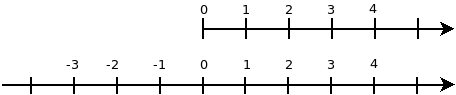
\includegraphics[width=13cm]{allg/alg/img/Zahlenstrahl.png}}
\end{center}

Der Zahlenstrahl hat den Startpunkt 0 (Null)\footnote{... manchmal  den Startpunkt 1 ...}, wohingegen die
Zahlengerade auf beiden Seiten uneingeschränkt weiterläuft.%%
}%% END TALS

\newpage


\subsection{Rationale Zahlen ($\mathbb{Q}$)}
\index{Zahlen!rationale}\index{rationale Zahlen}

\begin{definition}{rationale Zahlen}{}
Zahlen, welche sich als Bruch mit ganzen Zahlen schreiben lassen,
werden als \textbf{rationale Zahlen} bezeichnet.


$$\mathbb{Q} =\left\{ q = \frac{a}{b} \,\,\, \middle| \,\,\, a,b \in
\mathbb{Z}, b \ne 0 \right\}$$
\end{definition}

\subsubsection{Beispiele}

$$0.5 = \LoesungsRaum{\frac12} \hspace{1cm} (a=\LoesungsRaum{1}; b=\LoesungsRaum{2})$$

$$3 = \LoesungsRaum{\frac31} \hspace{1cm} (a=\LoesungsRaum{3}; b=\LoesungsRaum{1})$$

oder so:

$$-8 = \LoesungsRaum{\frac{-16}{2}} \hspace{1cm} (a=\LoesungsRaum{-16}; b=\LoesungsRaum{2})$$

$$0 = \LoesungsRaum{\frac{0}{7}} \hspace{1cm} (a=\LoesungsRaum{0}; b=\LoesungsRaum{7})$$


Mit den \textbf{rationalen} Zahlen sind uneingeschränkt durchführbar:
\begin{itemize}
\item Addition ($+$)
  \item Multiplikation ($\cdot$)
\item Subtraktion ($-$)
\item \LoesungsRaumLang{\textbf{Division} ($:$
  bzw. $\frac{\cdot{}}{\cdot{}}$ bzw. $\frac{\Box{}}{\Box{}}$)}
  \end{itemize}

\newpage


\subsubsection{Dezimalbrüche}\index{Dezimalbruch}
Jeder Bruch ($\frac{a}{b}$\TRAINER{  $a, b \in \mathbb{Z}, b\ne 0$}) lässt sich als
abbrechender oder periodischer Dezimalbruch schreiben. Beispiel:

Abbrechend:
$$\frac{175}{8} = \LoesungsRaumLang{21.875}$$
Periodisch:
$$\frac{5}{70} = \LoesungsRaumLang{0.0\overline{714285}}$$

Dasselbe gilt umgekehrt. Für abbrechende Dezimalbrüche ist dies
trivial:
$$47.386 = \LoesungsRaumLang{\frac{47\,386}{1\,000}}$$

Für periodische, nicht abbrechende
Dezimalbrüche\index{Dezimalbruch!periodisch}\index{periodische Dezimalbrüche} sieht die Sache etwas komplizierter aus,
gilt jedoch auch (sprich «Null Komma Periode Eins-Drei»):

$$0.\overline{13} = 0.131313... = \LoesungsRaumLang{13\cdot{}\frac1{99}=\frac{13}{99} = 13 : 99}$$

\TNTeop{Bem.: $\frac{1}{9} = 0.111\overline{1}$, $\frac{1}{99} = 0.0101\overline{01}$, $\frac{1}{999} = 0.001001\overline{001}$, ...}

%%%%%%%%%%%%%%%%%%%%%%%%%%%%%%%%%%%%%%%%%%%%

  \subsection*{Aufgaben}
  Zeigen Sie, dass die folgenden Dezimalzahlen rational sind. Schreiben Sie dazu diese Zahlen als gewöhnliche, gekürzte Brüche:

%%  \renewcommand{\arraystretch}{1.5}
  \begin{bbwFillInTabular}{|c|c|c|}
  $0.8=\LoesungsRaum{\frac45}$                  & $-2.03=\LoesungsRaum{-\frac{203}{100}}$         & $2.125=\LoesungsRaum{\frac{17}{8}}$                             \\
  $0.\overline{4} =\LoesungsRaum{\frac49}$      & $3.\overline{3}=\LoesungsRaum{\frac{10}{3} }$   & $4.\overline{16}=\LoesungsRaum{\frac{412}{99}}$
\end{bbwFillInTabular} 

  \TNTeop{
    Um einen Dezimalbruch in einen echten Bruch zu verwandeln, hilft
    der Taschenrechner. Periodische Dezimalbrüche werden so weit wie
    möglich repetitiv eingegeben.
    
\GESO{TI-30X Pro MathPrint: «Zahl»
  \tiprobutton{approx}\tiprobutton{enter}}
\TALS{TI nSpire CAS: «Zahl» -> Menu -> Zahl -> in Bruch approximieren}
  }

%%  \GESOAadBMTA{22}{Optional: 6., 7.}
%%  \TALSAadBMTA{8}{Optional: 1., 2.}

%%  \noTRAINER{\mmPapier{6}}%% END noTRAINER

%%%%%%%%%%%%%%%%%%%%%%%%%%%%%%%%%%%%%%%%%%%

\newpage

\subsection{Irrationale und reelle Zahlen ($\mathbb{R}$)}\index{Zahlen!reelle}

\youtubeLink{https://www.youtube.com/watch?v=9JgcETAN65c}{Simple-Club:
  Irrationale Zahlen}

\youtubeLink{https://www.youtube.com/watch?v=tPfnEByx9r0}{Dorfuchs: Wurzel zwei ist irrational.}

  Zahlen auf der Zahlengerade, welche nicht als Bruch $\frac{a}{b}$ mit $a\in\mathbb{Z}$, $b \in \mathbb{N}$ dargestellt werden können, werden als \textbf{irrational}\index{irrational} bezeichnet.

Wichtigste Vertreter:

\TNT{5.2}{\bbwCenterGraphic{12cm}{allg/alg/img/IrrationaleZahlen.png}}

\begin{definition}{Reelle Zahl}{}
Die Vereinigungsmenge der rationalen ($\mathbb{Q}$) und der irrationalen Zahlen
nennen wir die \textbf{reellen} Zahlen und bezeichnen die Menge mit $\mathbb{R}$.
\end{definition}


Dass $\pi$ oder $\sqrt{2}$ irrational sind, ist nicht trivial. Daher
noch zwei Vertreter irrationaler Zahlen, bei denen sofort klar ist,
dass es sich nicht um periodische Dezimalbrüche handelt:
\TNTeop{\begin{itemize}
\item $0.10 100 100010000100000100000010000000...$
\item $0.12345678910111213141516 ... 9899100101102103104 ... $
\end{itemize}%%
}%% END TNT

%%%%%%%%%%%%%%%%%%%%%%%%%%%%%%%%%%%%%%%%%%%%

\begin{gesetz}{Zahlmengen Beziehungen}{}
$$\LoesungsRaum{\mathbb{N}} \subset \LoesungsRaum{\mathbb{Z}} \subset
  \LoesungsRaum{\mathbb{Q}} \subset \LoesungsRaum{\mathbb{R}} $$%
\end{gesetz}


\begin{bemerkung}{Mächtigkeit}{}
  Dabei ist $\mathbb{R}$ die mächtigste der vier Mengen. 
\end{bemerkung}

\TNTeop{(Trainer: Beginne beim skizzieren mit $\mathbb{R}$)\\
\bbwCenterGraphic{8cm}{allg/alg/img/nzqr.png}
}%% END TNTeop

%%%%%%%%%%%%%%%%%%%%%%%%%%%%%%%%%%%%%%

\subsection*{Aufgaben zum Kapitel Zahlmengen}

\aufgabenFarbe{Geben Sie jeweils an, zu welchen der Zahlmengen $\mathbb{N}\backslash{}\{0\}$, $\mathbb{Z}$, $\mathbb{Q}$ bzw. $\mathbb{R}$ die folgenden Zahlen gehören:%%
}%% END Aufgabenfarbe

\begin{itemize}
\item $5-8 \LoesungsRaum{\mathbb{Z,Q,R}}$
\item $-3.\overline{17} \LoesungsRaum{\mathbb{Q,R}}$
\item $\sqrt{2.00} - \sqrt{\frac{50}{25}} \LoesungsRaum{\mathbb{Z,Q,R}}$
\item $\frac{3}{\pi} \LoesungsRaum{\mathbb{R}}$
\item $\sqrt{2^5}\LoesungsRaum{\mathbb{R}}$
\item $4.\overline{9} \LoesungsRaum{\mathbb{N,Z,Q,R}}$
\item $3.\overline{18}+\frac{20}{11} \LoesungsRaum{\mathbb{N,Z,Q,R}}$
\item $0.313113111311113111113... \LoesungsRaum{\mathbb{R}}$
\item $\sqrt{-6} \LoesungsRaum{\not\in\mathbb{R}}$
\end{itemize} 

%%\GESOAadBMTA{22ff}{5.}
%%\TALSAadBMTA{9}{4.}

\TNTeop{}
